\section{Apparato sperimentale}\label{sec:apparato-sperimentale}
Per questo esperimento abbiamo realizzato due circuiti.
I valori numerici della tensione e delle resistenze utilizzate sono riportati
in tabella \ref{tab:livelli-logici}.

\subsection{Schema del circuito (1-bit full adder)}\label{subsec:schema-circuito}
\begin{figure}[h]
  \begin{subfigure}[t]{.66\textwidth}
    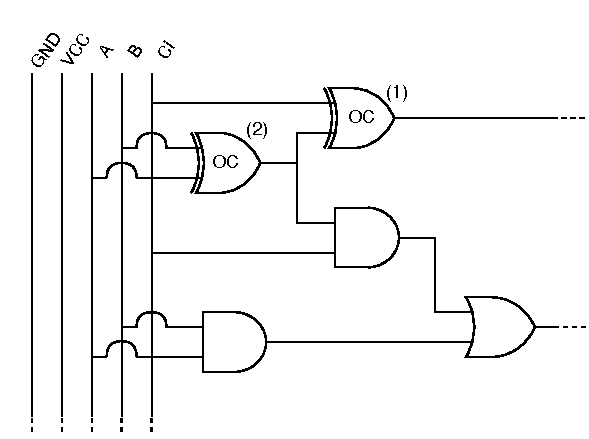
\includegraphics[width=10cm]{../assets/1bfa.drawio.pdf}
    \caption{
      \emph{
        Schema del circuito 1-bit full adder. Le iniziali "\textsc{oc}" sui gate \textsc{exor} indicano che i gate sono
        \emph{open collector}. In figura non sono riportate le resistenze di pull-up per i gate
        \textsc{exor}. $A$, $B$ e $C_i$ sono rispettivamente i due bit di input e il carry bit di input.
      }
    }
    \label{fig:circuito}
  \end{subfigure}
  %
  \hspace{5mm}
  %
  \begin{subfigure}[t]{.25\textwidth}
    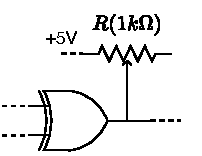
\includegraphics[width=5cm]{../assets/oc.drawio.pdf}
    \caption{
      \emph{
        Schema del collegamento dei gate \textsc{exor} alle resistenze di pull-up.
      }
    }
    \label{fig:exor-pullup}
  \end{subfigure}
  \caption{\emph{Schema circuitale per il circuito del full adder.}}
  \label{fig:circuiti}
\end{figure}

Il circuito che abbiamo realizzato è schematizzato in figura \ref{fig:circuito}.
Le porte logiche sono realizzate usando dei circuiti integrati e sono collegate tra di loro
in modo da rispettare le equazioni \eqref{eq:S} e \ref{eq:Co}.

\subsection{Schema del circuito (gate logici)}\label{subsec:schema-circuito-gate}
\begin{figure}[h]
  \begin{subfigure}[t]{.47\textwidth}
    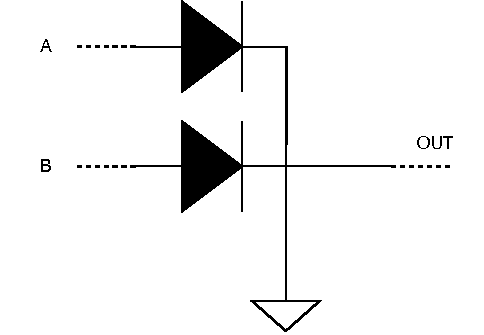
\includegraphics[width=7.75cm]{../assets/or.drawio.pdf}
    \caption{
      \emph{
        Schema del circuito per il gate \textsc{or}.
      }
    }
    \label{fig:or-gate}
  \end{subfigure}
  %
  \hspace{5mm}
  %
  \begin{subfigure}[t]{.47\textwidth}
    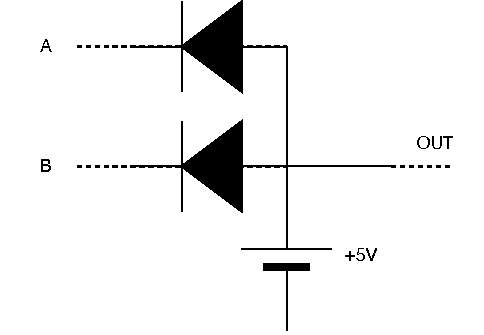
\includegraphics[width=7.75cm]{../assets/and.drawio.pdf}
    \caption{
      \emph{
        Schema del circuito per il gate \textsc{and}.
      }
    }
    \label{fig:and-gate}
  \end{subfigure}
  \caption{\emph{Schemi circuitali per simulare i gate logici. $A$ e $B$ sono gli input, $OUT$ è l'output.}}
  \label{fig:circuiti-gate}
\end{figure}

I circuiti che abbiamo realizzato sono schematizzati in figura \ref{fig:or-gate} e \ref{fig:and-gate}.

\subsection{Materiale e strumenti usati}\label{subsec:materiali}
Segue una lista del materiale e degli strumenti usati per entrambi i circuiti durante la prova:
\begin{itemize}
  \item%
  Multimetro digitale, modello: \emph{METEX M-3650D}.
  \item%
  Generatore di tensione, modello: \emph{ISO-TECH IPS 3303}.
  \item%
  Generatore di livelli logici, modello: \emph{Black Box}.
  \item%
  Connettori vari (connettori a banana, cavi per la scheda millefori).
  \item%
  Circuiti integrati per \textsc{or}, \textsc{and}, \textsc{exor}, rispettivamente modelli: \emph{7432}, \emph{7408}, \emph{74LS136}.
  \item%
  Due potenziometri da $1k\Omega$.
  \item%
  Resistenza da $10k\Omega$.
  \item%
  Due diodi al silicio, modello: \emph{1N4148}.
\end{itemize}

\begin{table}[H]
  \centering
  \begin{tabular}[t]{c | c  c }
    \hline
    Grandezza & Valore & Fondoscala \\
    \hline
    d.d.p. generatore & $(5.04 \pm 0.03) \: V$ & $20 \: V$ \\
    Resistenza 1 & $(410 \pm 5) \: \Omega$ & $2 \: k\Omega$ \\
    Resistenza 2 & $(356 \pm 5) \: \Omega$ & $2 \: k\Omega$ \\
    Stato basso F.A. & $(0.120 \pm 0.010) \: V$ & $2 \: V$ \\
    Stato alto F.A. & $(4.04 \pm 0.02) \: V$ & $20 \: V$ \\
    Stato basso circ.\\ logica positiva & $(0.000 \pm 0.010) \: V$ & $2 \: V$ \\
    Stato alto circ.\\ logica positiva & $(5.04 \pm 0.03) \: V$ & $20 \: V$ \\
    \hline
  \end{tabular}
  \caption{\emph{Grandezze caratteristiche dei circuiti.}}
  \label{tab:livelli-logici}
\end{table}
